\documentclass{report}
\usepackage[T1]{fontenc} % Fontes T1
\usepackage[utf8]{inputenc} % Input UTF8
\usepackage[style=numeric,sorting=none]{biblatex} % para usar bibliografia

\addbibresource{bibliografia.bib}
\usepackage{csquotes}
\usepackage[portuguese]{babel} %Usar língua portuguesa
\usepackage{blindtext} % Gerar texto automaticamente
\usepackage[printonlyused]{acronym}
\usepackage{hyperref} % para autoref
\usepackage{graphicx}
\usepackage{indentfirst}

\bibliography{bibliografia}


\begin{document}
%%
% Definições
%
\def\titulo{Projeto Final LABI2023}
\def\data{16 junho 2021}
\def\autores{Marta Pedrosa, Orlando Marinheiro, Luis Rodrigues, Hugo Dias}
\def\autorescontactos{(108115) marta.beatriz@ua.pt, (114060) orlandomarinheiro@ua.pt\\(114560) lcr@ua.pt, (114142) hugomdias@ua.pt}

\def\departamento{Dept. de Eletrónica, Telecomunicações e Informática}
\def\empresa{Universidade de Aveiro}
\def\logotipo{ua.pdf}
%
%%%%%% CAPA %%%%%%
%
\begin{titlepage}

\begin{center}
%
\vspace*{50mm}
%
{\Huge \titulo}\\ 
%
\vspace{10mm}
%
{\Large \empresa}\\
%
\vspace{10mm}
%
{\LARGE \autores}\\ 
%
\vspace{30mm}
%
\begin{figure}[h]
\center
\includegraphics{\logotipo}
\end{figure}
%
\vspace{30mm}
\end{center}
%

\end{titlepage}

%%  Página de Título %%
\title{%
{\Huge\textbf{\titulo}}\\ [10pt]
{\Large \departamento\\ \empresa}
}
%
\author{%
    \autores \\
    \autorescontactos
}
%
\date{\today}
%
\maketitle

\pagenumbering{roman}

%%%%%% RESUMO %%%%%%
\begin{abstract}
Neste trabalho foi-nos proposto o desenvolvimento de um web-site que tem como objetivo carregar imagens, armazenar e garantir o acesso ás mesmas.
Dentro do Web-Site foram implementadas diversas funções para o uso do utilizador tais como a upload, que permite a publicação de imagens no site. Estas são armazenadas e podem ser acessadas através de uma página (gallery) que regista as imagens numa base de dados através do nome do autor inibindo assim o plágio das mesmas.
Neste site foi desenvolvido um metodo que permite a interação com outros utilizadores, sendo possível comentar as imagens de maneira a notificar o autor de alguns ajustes nas imagens que podiam ser feitos ou só mesmo para elogiar o seu excelente trabalho.
Para tornar o site mais completo, é possível também classificar a imagem como sendo boa ou má (Like / Dislike) tornando o autor mais reconhecido pela comunidade e para que este possa expandir o seu talento como criador de imagens.


\end{abstract}


%%%%%%%%%%%%%%%%%%%%%%%%%%%%%%%
\clearpage
\pagenumbering{arabic}

%%%%%%%%%%%%%%%%%%%%%%%%%%%%%%%%
\chapter{Introdução}
\label{chap.introducao}

Neste trabalho seram abordados vários Temas e Subtemas
Este está dividido em quatro capítulos.
Depois desta introdução,
no \autoref{chap.Interface Web} é apresentada a interface da página e os seus componentes com as respetivas funções,
no \autoref{chap.Aplicação} é abordado a realização do programa internamente, as linguagens utilizadas e as suas funcionalidades. O \autoref{chap.Persistência} apresenta a realização de uma base de dados que serve armazenamento às imagens, 
no \autoref{chap.resultados} são apresentados os resultados obtidos,
sendo estes discutidos no \autoref{chap.analise}.
Os testes realizados são apresentados no \autoref{chap.testes} de maneira a tornar o site mais confiável e a evitar a presença de erros inesperados.
Finalmente, no \autoref{chap.conclusao} é apresentada a conclusão do trabalho.

\chapter{Interface Web}
\label{chap.Interface Web}
A interface Web é composta por 6 páginas Web (Upload / Gallery / Index / Register / Login / About / Process) tendo estas as suas própias funcionalidades que serão desenvolvidas ao longo deste capítulo.\\

\section{Upload}

    A função da página Upload é processar imagens escolhidas por o utilizador para o web site, sendo obrigatório a implementação do nome do usuário que quer adicionar a imagem e o respetivo nome da mesma. \\ [10pt]



\begin{figure}[h]
    \centering
    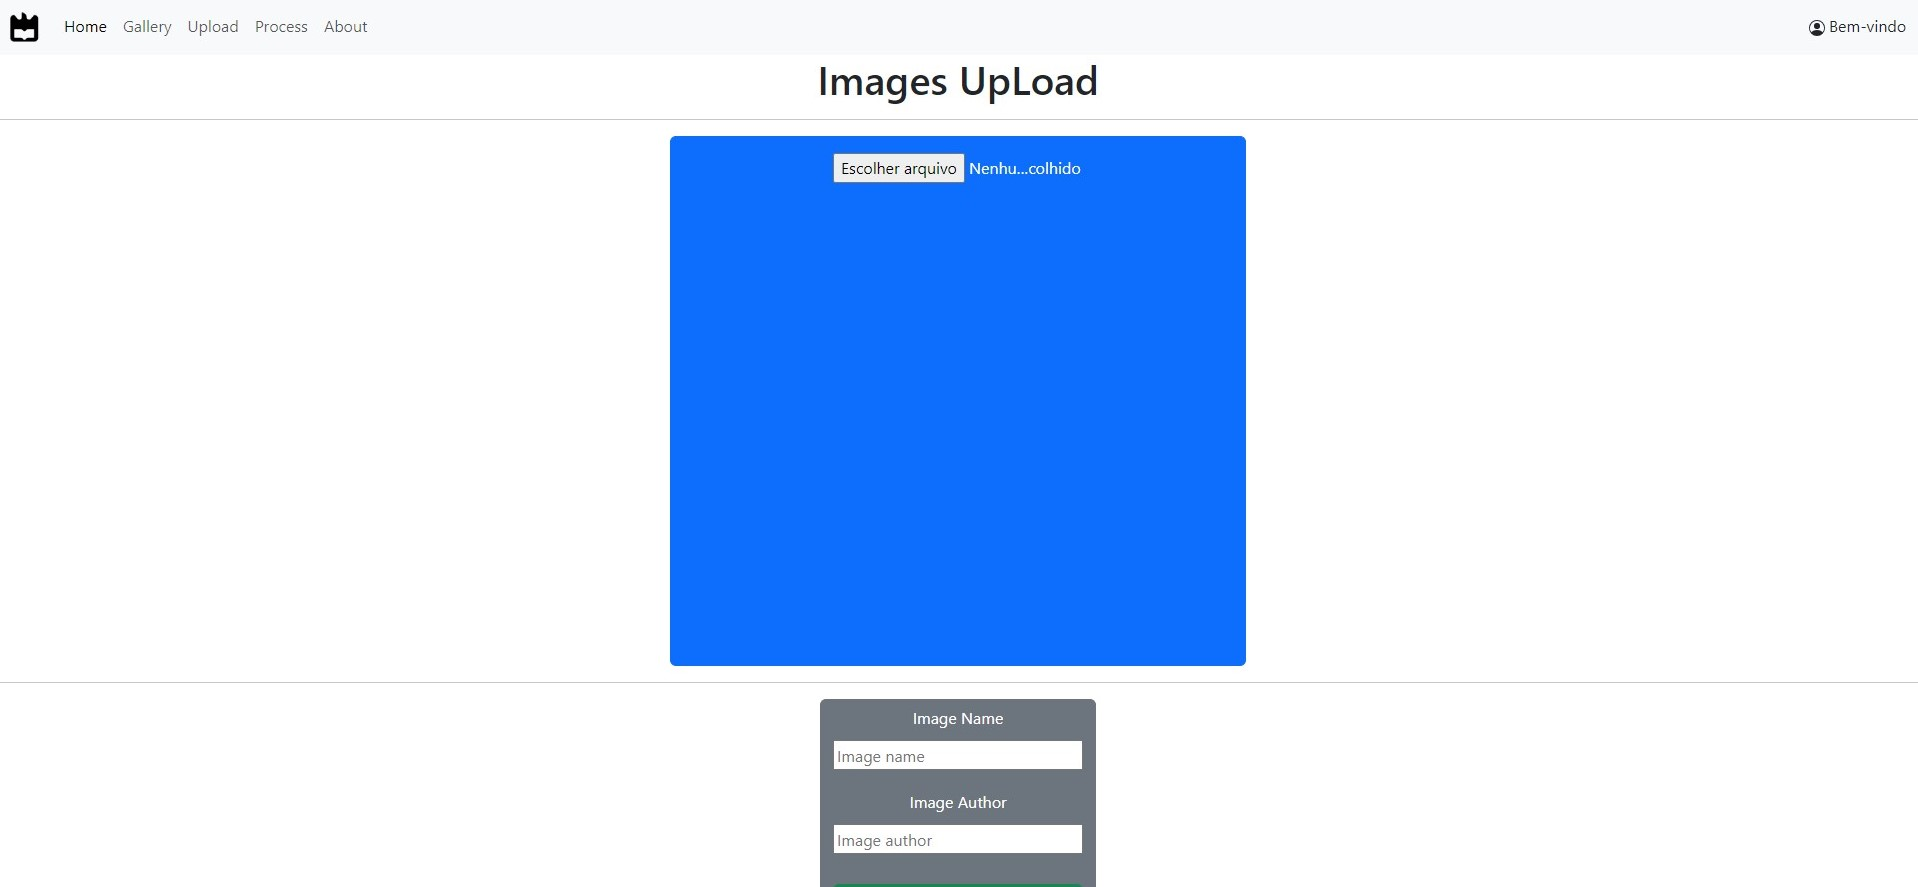
\includegraphics[width=\textwidth]{upload.jpg}
    \caption{Página do Upload}
\end{figure}

\section{Gallery}

    A página da Gallery é responsável por armazenar todas as fotos processadas no Web Site, sendo possível a sua filtração, ou por o nome do autor ou data adiconada ...
    Após a adição da imagem é possível carregar em cima da mesma e aceder a uma outra pagina dentro da gallery, onde poderá adicionar um comentário e classificar a imagem com um Like/Dislike.\\ [5pt]



\begin{figure}[h]
    \centering
    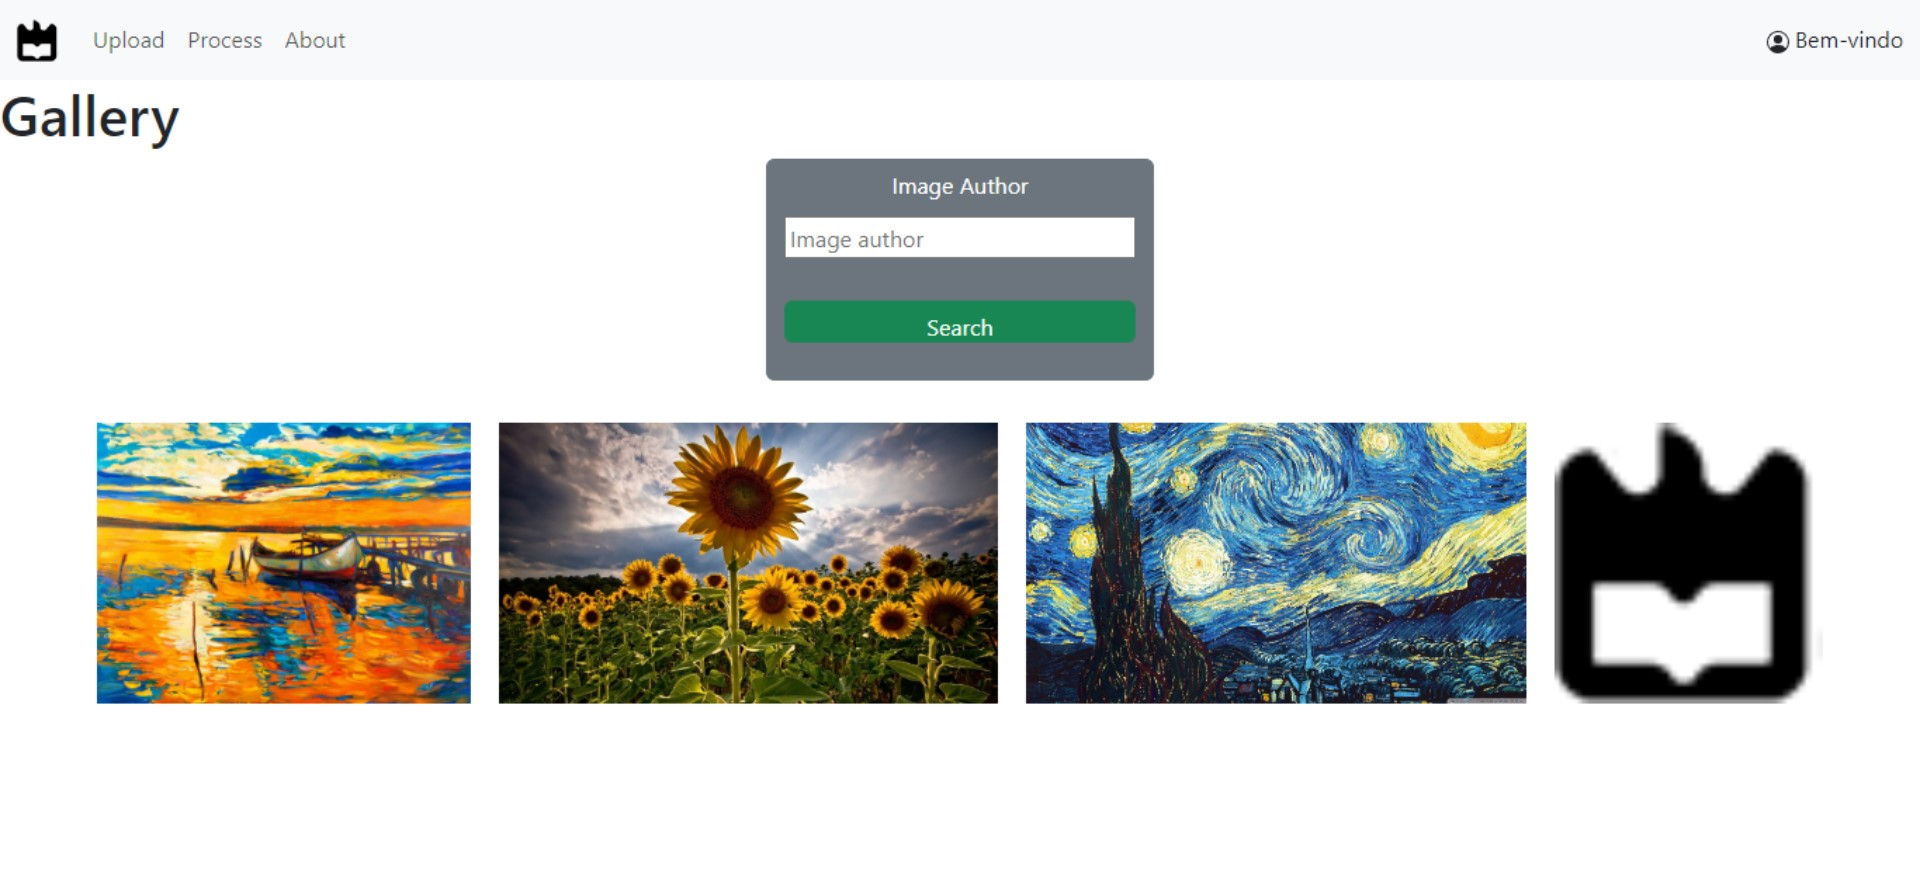
\includegraphics[width=\textwidth]{gallery.jpg}
    \caption{Página da gallery}
\end{figure}


\begin{figure}[h]
    \centering
    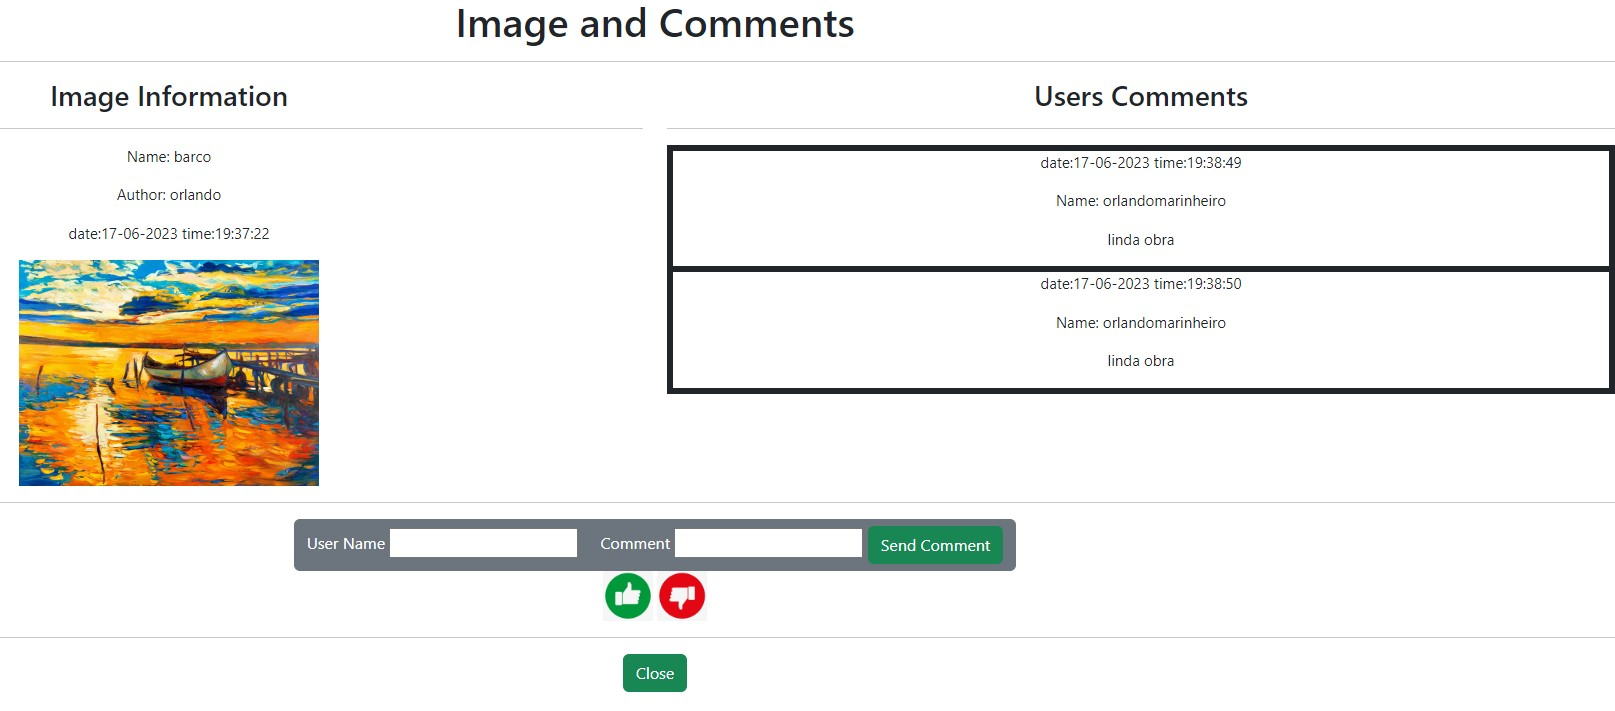
\includegraphics[width=\textwidth]{gallery2.jpg}
    \caption{Página da gallery2} 
\end{figure} 

\section{Process}

    A página Process permite ao user simular algoritmos de processamento de imagens, tais como redefinir o seu tamanho.
    
\section{About}

    A página About tem a simples função de fornecer os dados dos criadores e de uma forma sucinta dar a conhecer o objetivo do web site.

\section{Index}

    A página Index é a página introdutória do site, não tendo implementada nenhuma função, apenas é usada para dar boas vindas à pessoa que acabou de aceder.
    
\section{Registo / Login} 

    A página register é responsável por o registo de um utilizador com uma certa password escolhida, este armazena os dados do utilizador num ficheiro csv, que depois poderá ser acessado.

    A página login é responsável por dar acesso ao site também através de um nome de utlizador e de uma password já registada. No caso de um destes não estar presente no ficheiro csv, não lhe será permitido aceder ao site. 
    \\
\begin{figure}[h]
    \centering
    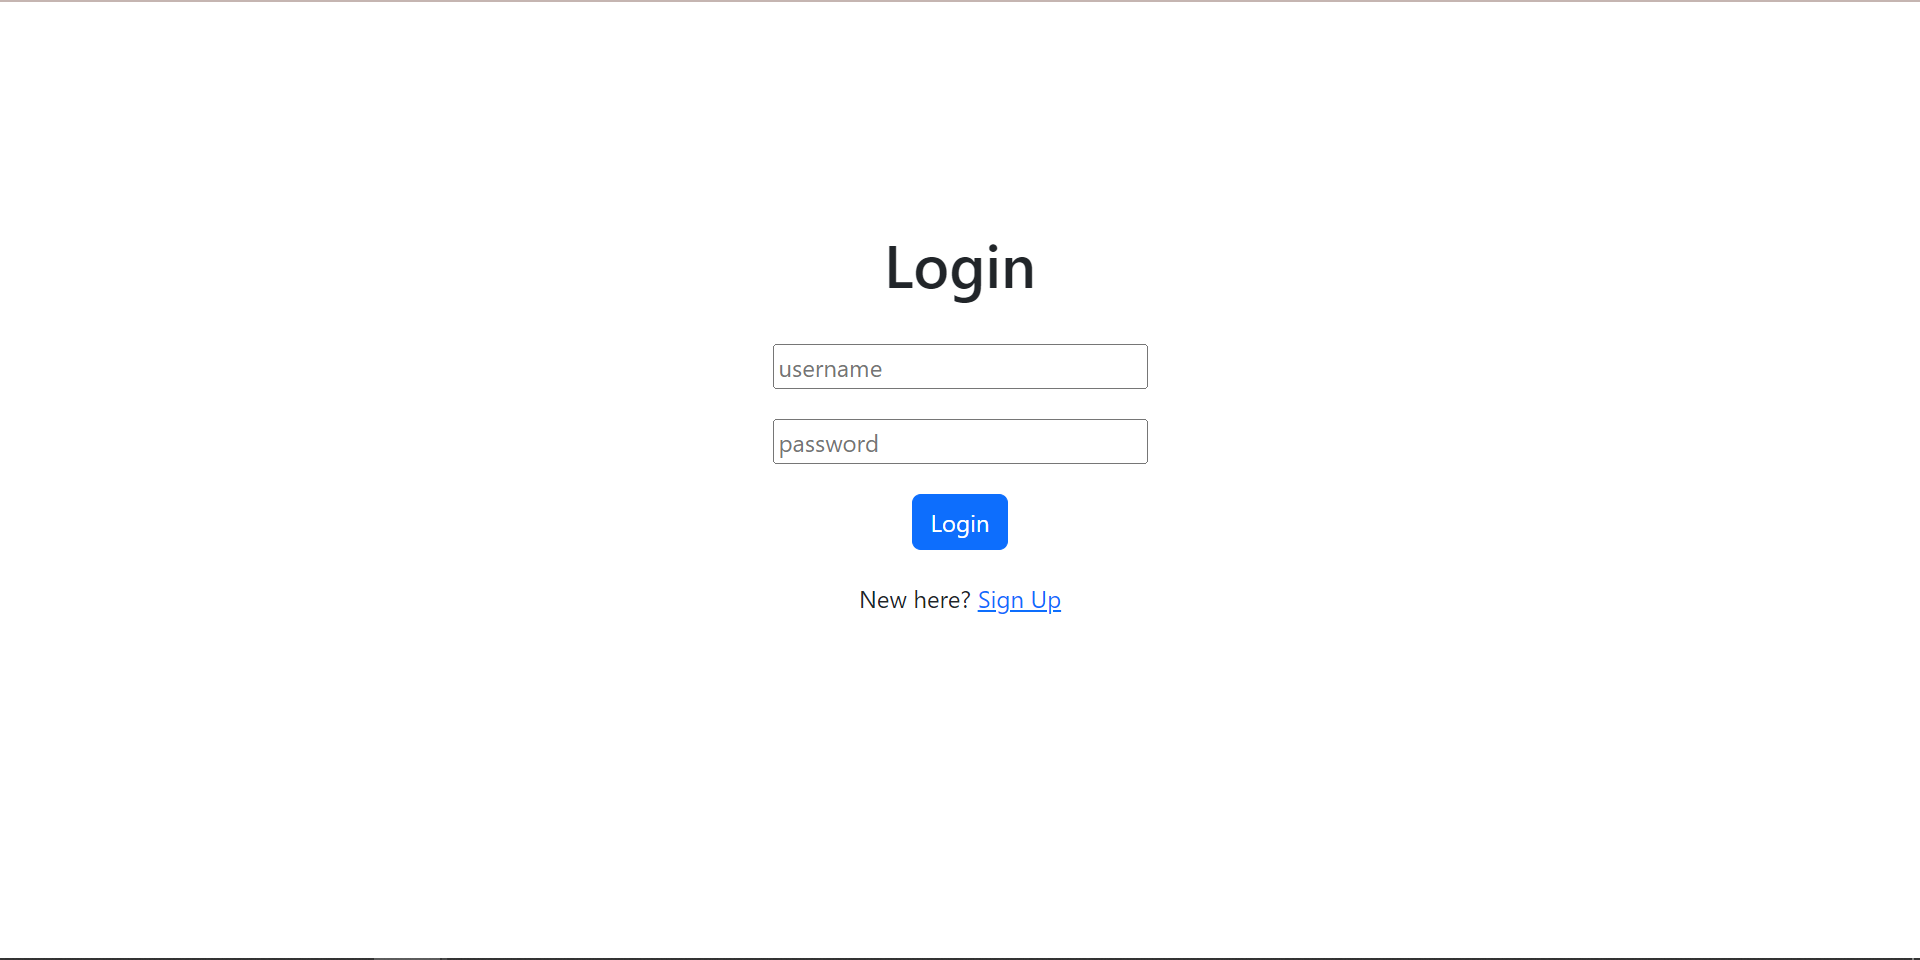
\includegraphics[width=\textwidth]{LoginPage.png}
    \caption{Página do Login}
\end{figure}

\chapter{Aplicação Web}
\label{chap.Aplicação}
Neste Web site, a Aplicação Web foi desenvolvida de uma forma apelativa e simples permitindo aos desenvolvidores do Web Site uma perceção intuitiva daquilo que outros fizeram
Para este desenvolvimento serviram como base recursos de JavaScript e Python para implementar as funções utilizadas nas páginas de processamento e armazenamento de imagens e também para o funcionamento do servidor.
Com o intuito de dar estrutura / criar o esqueleto do Web Site foi utilizada a Linguagem " HyperText Markup Language (HTML) " e por fim um pouco de CSS para tornar o site mais apelativo e agradável aos utilizadores .


\chapter{Persistência}
\label{chap.Persistência}
Este parâmetro é composto por uma base de dados, realizada em SQLITE3. 
Esta base de dados armazena todas as imagens enviadas pelo utilizador para o Web Site, possuindo toda a informação relativamente àquela imagem como o seu ID, o seu nome, o nome do Autor, a data de envio, o comentário ...


\chapter{Resultados}
\label{chap.resultados}
Como resultado final do Web Site conseguimos aceder ao mesmo atraves da inscrição de um usuário e o respetivo login. Já dentro do Site é possível adicionar uma imagem ao mesmo e regista-la com o seu nome e com o nome do seu autor (Upload), também se consegue aceder a uma galeria onde é possibilitada a visualização de todas as imagens processadas na Web, quer seja do usuário como de outros. Ao aceder a uma das imagens, conseguimos observar os seus dados como também publicar um comentário acerca da mesma e visualizar outros comentários. Na página about observamos a informação do Site e os seus criadores. 
Não está implementada a função Process nem a classificação da imagem (Like / Dislike).

\chapter{Análise}
\label{chap.analise}
Apesar de o Web Site não estar completo, as funções implementadas parecem fazer o seu trabalho corretamente sem qualquer problema.

\chapter{Testes}
\label{chap.testes}
Não foi realizado nenhum teste unitário, que permitiriam testar e evitar errosque poderiam gerar ao longo do percurso do seu desenvolvimento 

\chapter{Conclusões}
\label{chap.conclusao}
Com o desenvolvimento deste Site podemos concluir que, a realização do mesmo permitiu ter um pouco mais a noção de como realmente funciona a interação entre o utilizador e o computador. Este trabalho também nos proporcionou um aprofundamento e mais prática nas linguagens abordadas, como CSS, Html, Java Script e Python.
Foi possível também aprender mais sobre um campo na área da programção que são as bases de dados, acredito que não tenha sido usada no seu maior potencial porém deu para ter a noção do seu real valor neste universo da informática e o quanto é importante a sua presença numa aplicação ou Website interativo.
Apesar de alguns imprevistos na implementação do Web Site, a sua realização foi muito interessante e ajudou-nos a adicionar mais conhecimento ao nivel informático que futuramente poderá ser muito útil no mundo do trabalho ou na realização de projetos. 

\chapter*{Contribuições dos autores}
Este trabalho foi divido por todos os membros do grupo, tal que o \ac{HD} ficou por fazer o Relatório, a página about e o visual do site, O \ac{OM} realizou a página que regista e dá login aos utilizadores, a página Upload e a gallery e ajudou nos comentarios , o \ac{LR} e a \ac{MP} ajudaram nos comentarios e nos likes/dislikes.

\vspace{10pt}
\textbf{Indicar a percentagem de contribuição de cada autor.}\\

\autores : 10\%, 45\%, 10\%, 35\%\\

\textbf{Repositório GitHub:} labi2023g15

%%%%%%%%%%%%%%%%%%%%%%%%%%%%%%%%%
\chapter*{Acrónimos}
\begin{acronym}
\acro{ua}[UA]{Universidade de Aveiro}
\acro{HD}[HD]{Hugo Dias}
\acro{OM}[OM]{Orlando Marinheiro}
\acro{LR}[LR]{Luis Rodrigues}
\end{acronym}


%%%%%%%%%%%%%%%%%%%%%%%%%%%%%%%%%
\printbibliography

\end{document}